\section{ACPUserAuth}

Damit der Admin-Client vom Personal eines Restaurants benutzt werden kann, muss dieses sich mit 
einem gültigen ACP-Nutzer anmelden.\\
Anders als beim normalen Client kann hier kein ACP-Nutzer erstellt werden, dies muss über das
\nameref{acp} geschehen.

Dementsprechend sind auch zur Verwendung dieses Services die entsprechenden ACP-User-Routes nötig,
die, wie bereits bekannt, als statische Variablen innerhalb der Klasse gespeichert werden.

\begin{code}[H]
    \centering
    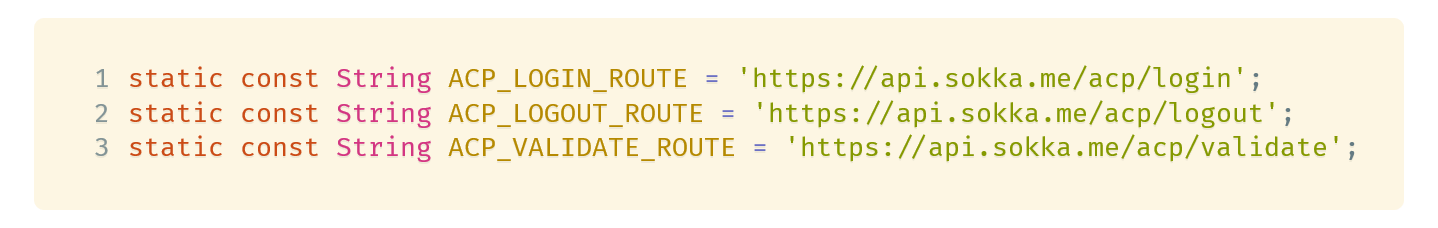
\includegraphics[width=1\textwidth]{images/Admin-Client/services/acpuserauth/acproutes.png}
    \vspace{-25pt}
    \caption{API-Routes für den User-Auth-Service}
\end{code}

Jene Routen werden in den jeweiligen Funktionen aufgerufen, um einen entsprechenden Request an
die den Server zu senden.